\chapter{Modelos Exponenciales de Grafos de Markov}
\label{ch:ERGMS}
\begin{chapquote}{Dr. Peter Clifford, \textit{The Royal statistical society meeting on the Gibbs sampler and other statistical Markov Chain Monte Carlo methods(1993)}}
``... from now on we can compare our data with the model we actually want to use rather than with a model which has some mathematically convenient form. This is surely a revolution.''
\end{chapquote}


\section{Introducción}


Para empezar a plantear el modelo final de esta tesis es necesario que pensemos que vamos a utilizar la probabilidad condicional para atacar un problema de un proceso espacial. Para esto es necesario que pensemos en los vecinos de cualesquiera que fuese nuestro grafo y que la probabilidad de que estos estén conectados tienen que ver con las conexiones de estos mismos al resto de los nodos del grafo.

\begin{figure}
    \centering
    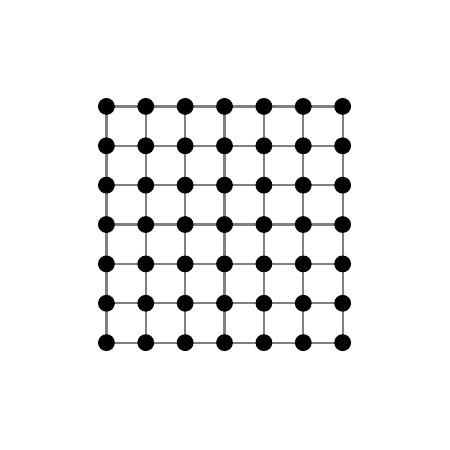
\begin{tikzpicture}
    \clip (-1,-1) rectangle (4cm,4cm); 
    \draw[style=help lines,thick] (0,0) grid[step=.5cm] (3,3);

    \foreach \x in {0,1,...,6}
    {
        \foreach \y in {0,1,...,6}
        {
            \node[draw,circle,inner sep=2pt,fill] at (.5*\x,.5*\y) {};
        }
    }

\end{tikzpicture}
    \caption{Un retículo cuadrado regular}
    \label{fig:retícula}
\end{figure}



Incluso si no estamos explícitamente interesados en cómo otros lazos afectan la probabilidad, los efectos del grafo implican una correlación de los residuos, por lo que ignorarlos producirá estimaciones sesgadas. Aquí hay un ejemplo intuitivo: si los EE. UU. y el Reino Unido están en guerra con Irak, ese hecho debe considerarse para una estimación imparcial de las probabilidades de que EE. UU. y el Reino Unido estén en guerra entre sí.

Para actuar más definidamente consideremos que restringimos nuestra atención a una retícula regular cuadrada con sus sitios (o nodos) denotados por los pares de números enteros $(i,j)$ asociadas a un conjunto de variables aleatorias $\{\mathcal{X}_{i,j}\}$. En este momento no es necesario pensar sobre la finitud de la retícula (\cite{Besag1974}). Entonces de acuerdo con \cite{Besag1974} la definición de función de distribución conjunta de las variables debería ser de la forma 

\begin{equation}
        \prod _ { i , j } Q _ { i , j } \left( x _ { i , j } ; x _ { i - 1 , j } , x _ { i + 1 , j } , x _ { i , j - 1 } , x _ { i , j + 1 } \right),
\end{equation}

donde $x_{i,j}$ es el valor de la variable aleatoria, $\mathcal{X}_{i,j}$. Sin embargo, es necesario que consideremos clases de probabilidad condicional más amplias en los cuales la distribución condicional de $\mathcal{X}_{i,j}$ se le permite depender de sitios más remotos. Podemos generalizar de tal forma que el esquema de (4.1) y cualquier generalización de éste será incluido. Esto es posible si extendemos el concepto de primer, segundo y cualquier orden de cadena de Markov en una dimensión al reino de los procesos espaciales. Esto es posible gracias a la demostración del teorema de Hammersley-Clifford.

A través de esta sección se van a examinar las limitaciones y problemas con el presente modelo y las implicaciones de derivar las funciones de probabilidad conjunta a partir de la estructura asociada del grafo. 



\section{Grafos Aleatorios de Markov}

%Una Grafo aleatoria de Markov es un modelo para un conjunto de variables X, donde las variables estan divididas en \textit{clans} $X_c$ y tenemos un factor $\Psi_c(X_c)$ esta definido para cada clan:

%$$\mathcal{P}(x) = \frac{1}{Z}\prod_{c=1}^C \Psi_c(X_c)$$

Un grafo aleatorio de Markov es resultado de un proceso aleatorio multidimensional que generaliza sobre un proceso de Markov de una sola dimensión como el de la Figura 4.2 a uno de múltiples dimensiones como el de la Figura 4.1.

\begin{figure}[Reticulo]
    \centering
    \begin{tikzpicture}
        % Setup the style for the states
        \tikzset{node style/.style={state, 
                                    fill=gray!40!white,
                                    circle}}

        \node[node draw=none, left=of II]               (I)   {};
        \node[node style, right=of I]   (II)  {$X_{i-1}$};
        \node[node style, right=of II]  (III) {$X_i$};
        \node[node style, right=of III] (IV)  {$X_{i+1}$};
        \node[draw=none,  right=of IV]   (V) {$\cdots$};
        

        \path[-stealth] (I) edge (II);
        \path[-stealth] (II) edge (III);
        \path[-stealth] (III) edge (IV);
        \path[-stealth] (IV) edge (V);

    \end{tikzpicture}
    \caption{Proceso de Markov 1D}
    \label{fig:Markov1D}
\end{figure}

    
\begin{definition}{Vecindario en el modelo de 2D}

En un retículo cuadrado regular un \textbf{vecindario} $\mathcal{N}(X_{i,j}) = \{x_{i-1,j},x_{i+1,j},x_{i,j-1},x_{i,j+1}\}$. Este vecindario de primer orden consiste de los vecinos de arriba, abajo, izquierda y derecha. 
    
\end{definition}



\section{Teorema de Hammersley-Clifford}

Suponemos que estamos interesados en una colección finita de variables aleatorias $X_1, \dots ,X_n$ que están asociadas con los nodos $1,\dots,n$ respectivamente. Para cada nodo, \\ $\mathcal{P}(x_i|x_1,\dots,x_{i-1},x_{i+1},\dots,x_n)$ es la distribución condicional de $X_i$ dado todos los otros valores, está especificada y necesitamos la probabilidad conjunta de todas las otras variables aleatorias.

Asumimos que si $x_1,\dots,x_n$ pueden ocurrir individualmente en los sitios $1,\dots,n$, respectivamente, pueden ocurrir juntos. Formalmente, si $\mathcal{P}(x_i) > 0$  $\forall$  $i $, entonces $\mathcal{P}(x_1, \dots, x_n) > 0$. Hammersley y Clifford (1971) exige a la condición de positividad  y se asumirá a lo largo de esta tesis. Además también es usual en la práctica. Definimos el espacio muestral $\Omega$ como el conjunto de todas las realizaciones posibles $\mathbf { x } = (x_1, ..., x_n)$ del sistema. Es decir, $\Omega = \{\mathbf { x }: P (\mathbf { x })> 0\}$. Entonces se sigue que para dos realizaciones dadas $\mathbf { x }$ y $\mathbf { y } \in \Omega$,


\begin{equation}
        \frac {P(x)} {P(y)} =
        \prod _ { i = 1 } ^ { n } \frac { P \left( x _ { i } | x _ { 1 } , \ldots , x _ { i - 1 } , y _ { i + 1 } , \ldots , y _ { n } \right) } { P \left( y _ { i } | x _ { 1 } , \ldots , x _ { i - 1 } , y _ { i + 1 } , \ldots , y _ { n } \right) }
\end{equation}

La prueba de esta igualdad está basada sobre el hecho que en nuestro caso podemos escribir

\begin{equation}
        P ( \mathbf { x } ) = P \left( x _ { n } | x _ { 1 } , \ldots , x _ { n - 1 } \right) P \left( x _ { 1 } , \ldots , x _ { n - 1 } \right)
\end{equation}

sin embargo $P \left( x _ { 1 } , \ldots , x _ { n - 1 } \right)$ no puede ser factorizado de una forma útil, de hecho $P \left( x_{n-1} | x _ { 1 } , \ldots , x _ { n - 2 } \right)$ no es fácilmente obtenido de las distribuciones condicionales dadas. Sin embargo podemos introducir $y_n$

\begin{equation}
    \begin{split}
        \begin{array} { c } { P ( \mathbf { x } ) = \frac { P \left( x _ { n } | x _ { 1 } , \ldots , x _ { n - 1 } \right) } { P \left( y _ { n } | x _ { 1 } , \ldots , x _ { n - 1 } \right) } P \left( x _ { 1 } , \ldots , x _ { n - 1 } , y _ { n } \right). } \end{array}
    \end{split}
\end{equation}


Ahora podemos operar sobre $x _ { n - 1 }$ en  $P \left( x _ { 1 } , \ldots , x _ { n - 1 } , y _ { n } \right)$ y después de introducir $y_{n-1}$ de la misma forma tenemos que

\begin{equation}
\begin{split}
        { P \left( x _ { 1 } , \ldots , x _ { n - 1 } , y _ { n } \right) &= \dfrac { P \left( x _ { n - 1 } | x _ { 1 } , \ldots , x _ { n - 2 } , y _ { n } \right) } { P \left( y _ { n - 1 } | x _ { 1 } , \ldots , x _ { n - 2 } , y _ { n } \right) } \\ & \times P \left( x _ { 1 } , \ldots , x _ { n - 2 } , y _ { n - 1 } , y _ { n } \right) }.
\end{split}
\end{equation}

Si continuamos este proceso de refactorización eventualmente llegamos a la misma ecuación que (4.2) que determina la estructura de la función de probabilidad conjunta en términos de las condicionales dadas. Requerimos la condición de positividad para asegurar que los elementos del denominador sean distintos a cero.

Además, el lector astuto se habrá dado cuenta que como los sitios están asignados de forma arbitraria en realidad existen muchas factorizaciones de $\frac{P(x)}{P(y)}$ todas equivalentes y esto por lo tanto implica la existencia de severas restricciones sobre la forma funcional de las condicionales para poder llegar a algo matemáticamente consistente. A continuación elaboramos sobre la forma funcional de la función de distribución y vamos a demostrar el teorema de \cite{MonteCarloMethods}.




\subsection{Requisitos y preliminares}

\begin{definition}{Conjunto de vecinos.}
Se dice que el nodo j ($\neq i)$ es un vecino de i si y sólo si es que la forma funcional de $\mathcal{P}(x_i|x_1,\ldots,x_{i-1},x_{i+1},\ldots,x_n)$ es dependiente de la variable $x_j$. Formalmente se dice que si tenemos un grafo $\mathcal{G}(\mathcal{N},\mathcal{E})$ entonces  $N(X_i)$, el \textbf{conjunto de vecinos} de $X_i$, es tal que $X_j \in N(X_i)$ si y sólo si $\{X_i, X_j\} \in \mathcal{E}$.

Se va a utilizar $N(x_{ij})$ para denotar a los vecinos de $x_{i,j}$. 
\begin{example}
    En una retícula cuadrada regular tendríamos que
    $N(x_{i,j}) = \{x_{i,j-1},x_{i-1,j},x_{i,j+1},x_{i+1,j}\}$.
\end{example}



\end{definition}

\begin{definition}{Clan.}
    Cualquier conjunto de sitios que consistan de un sólo sitio o los conjuntos de sitios en los cuales cada uno de sus elementos es vecino de cada otro elemento del conjunto.
    
    Formalmente decimos que $\mathcal{C} \subset \mathcal{N}$ es un \textbf{clan} si y solo si $\mathcal{C} \subset \{X,N(X)\}$ $\forall$ $X \in \mathcal{C}$.
\end{definition}

\begin{example}
    En una retícula regular y cuadrada como la de la figura 4.1 se dice que existen clanes de \{(i,j)\}, \{(i,j),(i-1,j\} y \{(i,j),(i,j-1)\}
\end{example}

\begin{definition}{Campo de Markov}
    
    Un \textbf{campo aleatorio de Markov} es una distribución de probabilidad sobre las variables  $x _ { 1 } , \ldots , x _ { n } $ definidas por un grafo no dirigido $G$ en los cuales los nodos corresponden a variables $ x _ { i }$. La probabilidad tiene la forma \\ 
    $${ \qquad \mathcal{P} \left( x _ { 1 } , \ldots , x _ { n } \right) = \frac { 1 } { Z } \prod _ { \mathrm { c } \in C } \phi _ { c } \left( x _ { c } \right) } $$
    donde $C$ denota el conjunto de clanes (i.e. los subgrafos totalmente conectados de G) y donde cada factor es una función no negativa sobre las variables que están contenidas en el clan. La función de partición está definida como\\ 
    $${ \qquad Z = \sum _ { x _ { 1 } , \ldots , x _ { n } } \prod _ { c \in C } \phi _ { c } \left( x _ { c } \right) }.$$ \\ 
    Entonces dado un grafo G nuestra función de distribución de probabilidad puede contener factores en los que no necesitamos especificar un factor para cada clan. %se dice clan
    Es decir que podríamos elegir clanes que contengan dos nodos (una relación de conectividad) pero no especificar ninguna que contenga factores unitarios.
    
    


\end{definition}

Ahora, para la demostración del Teorema de Hammersley-Clifford sólo debemos asumir dos premisas. Primero, supondremos que existen un número finito de valores disponibles a cada sitio, aunque esta condición se puede relajar si es necesario. Segundo, asumiremos que el valor cero está disponible en cada sitio. Si esto no fuese cierto, en realidad debido a la arbitrariedad de la asignación original simplemente podríamos reindexar nuestros valores en cada sitio de la retícula. Esta segunda premisa se utiliza simplemente para que podamos asegurar que bajo la condición de positividad tenemos que una realización de ceros es posible i.e. $P(0)>0$ y que podemos definir sin miedo a 

\begin{equation}
        Q(x) \equiv \ln \{P(x)/P(0)\}
\end{equation}

para cualquier $x \in \Omega$.

La pregunta que Hammersley y Clifford estaban intentando contestar es la siguiente: ¿Dado el conjunto de vecinos de cada sitio, cuál será la forma más general que $Q(x)$ puede tomar manteniendo una estructura de probabilidad válida al sistema?

Notamos que 

\begin{equation}
    \begin{split}
        \begin{aligned} \exp \left\{ Q ( \mathbf { x } ) - Q \left( \mathbf { x } _ { i } \right) \right\} & = \dfrac{P ( \mathbf { x } )} { P \left( \mathbf { x } _ { i } \right)} \\ 
        &= \dfrac{P \left( x _ { i } \; | \; x _ { 1 } , \ldots , x _ { i - 1 } , x _ { i + 1 } , \ldots , x _ { n } \right) }{ P \left( 0 \; | \; x _ { 1 } , \ldots , x _ { i - 1 } , x _ { i + 1 } , \ldots , x _ { n } \right)}  \end{aligned}
    \end{split}
\end{equation}

entonces la solución a este problema en realidad ya tiene la forma más general que puede ser tomada por la distribución de probabilidad condicional en cada sitio.


El método original de esta demostración requería el desarrollo de un cálculo operacional. Afortunadamente existe una prueba alternativa en donde la observación que para cualquiera distribución de probabilidad $P(X)$, sujeta a las condiciones establecidas, existe una expansión de $Q(X)$, única en $\Omega$ y de la forma


    \begin{equation}
        \begin{split} 
        Q ( x ) &= \sum _ { 1 \leq i < n } x _ { i }  \cdot G _ { i } \left( x _ { i } \right) + \sum _ { 1 < i < j \leqslant n } x _ { i } x _ { j } \cdot G _ { i j } \left( x _ { i } , x _ { j } \right)\\
        &+  \sum \sum _ { 1 \leqslant i < j < k \leqslant n} \sum _ {  } x _ { i } x _ { j } x _ { k } \cdot G _ { i , j , k } \left( x _ { i } , x _ { j } , x _ { k } \right) + \ldots \\ 
        &+ x _ { 1 } x _ { 2 } \ldots x _ { n } \cdot G _ { 1,2 , \ldots n } \left( x _ { 1 } , x _ { 2 } , \ldots , x _ { n } \right) 
        \end{split}
        \end{equation}


Con esta notación establecida podemos decir que el resultado de Hammersley-Clifford puede ser puesto de la siguiente forma

\begin{theorem}{Hammersley-Clifford}

    Definimos un grafo $\mathcal{G}(\mathcal{N},\mathcal{E})$ tal que $\mathcal{N} = \{X_1, \ldots, X_n\}$. Tenemos que $\{X_i,X_j\} \in \mathcal{E}$ si y sólo si\\
    $$\mathcal{P} ({x_i| \{x_1,\ldots,x_n\} - \{x_i\}) \neq \mathcal{P}(x_i | \{x_1,\ldots,x_n\} - \{x_i, x_j\} ).$$

    Para cualquier $1 \leq i < j < \dots < s \leq n$, la función $G_{i,j,\dots,s}$ en (4.8) que es una expansión única de $Q(x)$ definida en (4.6) debe de ser no nula si y sólo si los sitios elegidos $i,j,\dots,s$ forman un clan. Sujeto a esta restricción, las funciones G pueden ser elegidas arbitrariamente. Entonces, dados los vecinos de cada sitio, podemos inmediatamente escribir la forma más general para $Q(x)$ y por lo tanto para distribuciones condicionales.\\
    
    Demostración: se sigue de la ecuación (4.7) que para algún $x \in \Omega$, se tiene que $Q(x) - Q(x_i)$ sólo puede depender de $x_i$ en sí y los valores en los sitios que son vecinos del sitio $i$. Sin pérdida de generalidad, consideramos el sitio 1 en detalle. De aquí se obtiene la ecuación
    
    
   \begin{equation}
       \begin{split}
           Q(X) - Q(X_i) &= x_1 \left(G_1(x_1) + \sum_{2 \leq j \leq n} x_j G_{1j}(x_1,x_j) \\
           & + \sum_{2 \leq j < k < n} x_j x_k G_{1,j,k} (x_1,x_j,x_k) \\
           &+ \ldots + x_2 x_3 \cdots x_n G_{1,2,\ldots,n}(x_1,x_2,\ldots,x_n) \right )
       \end{split}
   \end{equation}
        

       %HELP ME fix this%
    
    Ahora suponemos que el sitio $l (\neq 1)$ no es un vecino del sitio 1. Entonces $Q(x)-Q(x_1)$ debe de ser independiente para todos los $x \in \Omega$. Fijando $x_i = 0$ para $i \neq 1$ o $l$, inmediatamente se nota que $G_{1,l}(x_1, x_l) = 0$ en $\Omega$. Asimismo, con otras decisiones prudentes de $x$, es fácil ver que sucesivamente todas las funciones de G de 3,4,$\dots$,n variables que incluyan tanto $x_1$ como $x_l$ deben de ser nulas. El resultado es análogo para cualesquiera dos sitios que no sean vecinos uno del otro, en general $G_{i,j,\dots,s}$ puede ser no nulo si los sitios $i,j,\dots,s$ forman un clan i.e.
    
    $$G_{i,j,\ldots,s}(x_i,x_j,\ldots,x_s) \neq 0 \iff \{i,j,\ldots,s\} \in cl(\mathcal{G}).$$
    
    Por el otro lado, cualquier conjunto de G-funciones da lugar a distribuciones válidas de $P(x)$ lo cual satisface la condición de positividad. También, como $Q(x)-Q(x_i)$ sólo depende de $x_l$ si existe una función no nula de G que involucre ambos $x_i$ y $x_l$ entonces se sigue que esto también es cierto de $P(x_i|x_1,\dots,x_{i-1},x_{i+1},\dots,x_n)$.
    
    Con esto queda demostrado el teorema.

\end{theorem}

Bajo la condición de positividad tenemos que : 

$${ \qquad \mathcal{P} \left( x _ { 1 } , \ldots , x _ { n } \right) = \frac { 1 } { Z } \prod _ { \mathrm { c } \in C } \phi _ { c } \left( x _ { c } \right) } $$

y por el Teorema de Hammersley-Clifford tenemos que lo siguiente es equivalente a (\cite{HCTheoremImpact}), 

\begin{itemize}
    \item \textbf{Propiedad local de Markov}: $\mathcal{P}(x_i|x-\{x_i\}) = \mathcal{P}(x_i|N(x_i))$ .
    \item \textbf{Propiedad de factorización}: La probabilidad se factoriza de acuerdo a los clanes del grafo.
    \item \textbf{Propiedad global de Markov}: $\mathcal{P}(x_A|x_B,x_S) = \mathcal{P}(x_A|x_S)$ cuando $x_A$ y $x_B$ están separados por $x_S$ en $\mathcal{G}$.
\end{itemize}

De hecho, lo que es realmente de interés para nosotros es un corolario relativamente simple del teorema (\cite{MonteCarloMethods}).

\begin{corollary}
    Para cualquier campo de Markov\\
    $$P(X_i = x_i, X_j = x_j, \dots, X_s = x_s| \text{Todos los otros sitios} )$$
    
    depende únicamente de $x_i,x_j,\dots,x_s$ y los valores de los sitios vecinos de los sitios $i,j,\dots,s$. En términos de Hammersley-Clifford se dice que las propiedades Markovianas globales y locales son equivalentes.
\end{corollary}

\section{Modelos exponenciales de grafos aleatorios}


Los modelos exponenciales de grafos aleatorias (\textit{ERGMs}) son una clase de modelos como las regresiones lineales son una clase de modelos. La forma general del modelo especifica la probabilidad de nuestro grafo (de lado izquierdo), como una función de términos que representan las características de nuestro grafo. Nuestra hipótesis inicial es que estas estadísticas descriptivas son suficientemente buenas para describir a nuestro grafo. La forma general es de la siguiente forma:

$$P(Y = y) = \frac{e^{\theta^{'}g(y)}}{\mathcal{Z}(\theta)}.$$

En este caso decimos que \mathcal{Y} es la variable aleatoria para el estado del grafo (con realización $y$),
$g (y)$ es un vector de estadísticas globales del grafo $y$, $\theta$ es el vector de coeficientes para esas estadísticas y $\mathcal{Z} (\theta)$ representa la cantidad de grafos posibles (normalmente restringida a todas los grafos posibles con el mismo número de nodos establecido en $y$).

La familia de grafos aleatorios exponenciales son una forma general de la clase de modelos de la familia exponencial en que especifican la función de distribución de probabilidad para un conjunto de grafos. Podemos definir modelos para grafos que incluyan variables que representen características como tríadas y homofilía, mutualidad, y una variedad de elementos estructurales de interés.

Con los ERGMs podemos obtener los estimadores de máxima verosimilitud para los parámetros de un modelo específico dado un conjunto de datos. Podemos hacer experimentos sobre parámetros específicos dado un conjunto de datos y también podemos simular nuevos grafos basados en las estadísticas de los modelos mejor ajustados:



$$\log \left( \exp \left( \theta ^ { \prime } g ( y ) \right) \right) = \theta _ { 1 } g _ { 1 } ( y ) + \theta _ { 2 } g _ { 2 } ( y ) + \ldots + \theta _ { p } g _ { p } ( y ).$$

\section{El modelo $p*$ para grafos}

Consideremos un grafo dirigido sobre el conjunto de N nodos. Sobre este grafo vamos a mantener en mente las relaciones de emparejamiento sobre los nodos de nuestro grafo.

Tendremos que ser cuidadosos con los resultados de nuestra reducción sobre el cambio en nuestro grafo con el modelo $p*$ y los \textit{ERGMs}. Pues a pesar que de que estos grafos permiten que los actores sigan generalizaciones mas allá de la dependencia diádica de los modelos $p_1$ y que permiten que los modelos se construyan de forma estructural a partir del comportamiento social aún tienden a ser bimodales e inestables con números de nodos más grandes.


\subsection{Definiendo estadísticas para el modelo $p*$}

Las estadísticas $g(y)$ pueden considerarse como las covariables del modelo. En el contexto del modelado de grafo, estas representan distintas características del grafo como densidad, homofilia, tríadas, etc. En cierto sentido, son como variables que se podrían usar en otros modelos estadísticos. Pero son diferentes en un aspecto importante: estas estadísticas $g(y)$ son funciones del grafo en sí, cada una se define por la frecuencia de una configuración específica de medidas observadas en el grafo, por lo que no se miden por una pregunta que se incluya en una encuesta (por ejemplo, el ingreso o cualquier atributo de un nodo), pero en su lugar debe calcularse en la grafo específica que se tiene, después de haber recopilado los datos.

Aquí es de suma importancia considerar a estadísticas que causan otro tipo de dificultades más adelante pero resultan ser de mucha importancia pero de poca conveniencia como las tripletas transitivas y el número de aristas:

$$u_{1}(y)=\sum_{i, j, h} y_{i j} y_{j h} y_{i h}$$
$$u_{2}(y)=y_{++}=\sum_{i, j} y_{i j}$$



En parte es por el uso de estadísticas que se propagan por todo el grafo y hacen que los clanes recubran todo nuestro espacio que nuestras distribuciones finales tienden a ser bimodales. 




\subsubsection{Consecuencias de la selección de estadísticas}

Afortunadamente sabemos que cualquier modelo de un grafo puede ser expresado a través de la familia exponencial con algún número de estadísticas de sumas. Sin embargo tenemos que considerar que existen $n(n-1)/2$ parámetros que se relacionan con la reciprocidad. 

Siguiendo a \cite{Snidjers2010}, imponemos una condición de homogeneidad al igualar parámetros cuando se refieren al mismo tipo de configuración en el grafo. Por ejemplo en una grafo social de amistades, cuando consideramos reciprocidad pensemos que Alberto tiende a hacer amistades recíprocas pero que María tiende a ser más cautelosa con las personas que intentan ser sus amigos. Por el propósito de simplificar el modelo asumimos que existe una sola tendencia de reciprocidad que comparten María y Pedro.

Esto se llama \textbf{homogeneidad de configuraciones de grafos isomorfos} donde los parámetros están igualados si las configuraciones son iguales cuando ignoramos los índices de los grafos. 

También podemos ser menos radicales si es que podemos medir las características de los nodos que los llevan a ser más recíprocos en sus amistades y así podemos hacer que el efecto dependa de los atributos de los nodos.

\subsection{Estabilidad bajo selección de parámetros}

Lo que estamos buscando es si es que podemos replicar los características globales de un grafo a partir de las propiedades locales que tienen nuestros nodos y aristas. Entonces si pensamos en el modelo específico de un grafo de contenido relacional entonces podríamos esperar que los triángulos sean buenos indicadores con un elemento de reciprocidad y transitividad en la estadística. Podemos también extender este concepto a los elementos de k-estrellas cuyas figuras se pueden observar más adelante en esta tesis.

\cite{Snidjers2002} trata con esta problemática de selección de parámetros y es por eso que cuando estamos pensando en hacer un método de máxima pseudo verosimilitud que opera al maximizar la así llamada pseudo verosimilitud definida para los grafos dirigidos:

\begin{equation*}
    \ell(\theta)=\sum_{i, j} \ln \left(\mathrm{P}_{\theta}\left\{Y_{i j}=y_{i j} | Y_{h k}=y_{h k} \text { para todo }(h, k) \neq(i, j)\right\}\right).
\end{equation*}

\subsection{Limitaciones y consideraciones del modelo $p*$}

Existen una variedad de limitaciones al modelo de \textit{ERGM} que no únicamente tienen que ver con nuestra capacidad computacional o en nuestro caso la capacidad de explorar adecuadamente el espacio de probabilidades con el algoritmo de Gibbs. El modelo tiende a tener sesgos hacia el caso del grafo vacío o el grafo completo de acuerdo a cómo estamos condicionando nuestro modelo. Éstas se pueden arreglar haciendo que fijemos el número de aristas al igual que fijamos el número de nodos.

Parte de la complicación en la descripción de los fenómenos sociales es que tenemos muchos espacios vacíos en nuestras matrices de adyacencia y se vuelven esparcidas (que lleva a el mal condicionamiento) y además en grafos sociales de interés el número de nodos lleva a que el espacio de probabilidades se vuelva más grande.

Los términos que son independientes por díadas como los términos de homofilia nodal implican no dependencia entre diadas y por lo tanto la presencia o no presencia de una arista puede depender de los atributos del nodo pero no en la presencia de aristas conectadas a éste. Los términos dependientes de las aristas como los términos de grado o de tríadas, en contraste introducen efectos de dependencia entre nodos. Estos términos tienen efectos muy distintos a los anteriores y mucho de lo que es diferente en el modelaje de grafos sociales es a partir de estas medidas. Pues éstas introducen efectos cascada o ciclos de retroalimentación positivos y negativos que llevan a conclusiones contra intuitivas y a efectos altamente no lineales. Por lo tanto un modelo con medidas dependientes de aristas requieren un algoritmo de estimación distinto para que podamos observar distintos componentes.


Además en la estimación de los parámetros para distintos tipos de k-estrellas o k-triángulos, que en general tienden a tener soluciones más estables por los elementos de reciprocidad (\cite{BirdsFeather}),  es importante tener en mente, por ejemplo, que cuando incorporamos modelos que incluyan triángulos de 3 nodos estos mismos van a tener que llevar a la creación de más aristas


\begin{minipage}{.25\linewidth}
\begin{figure}[H]\centering

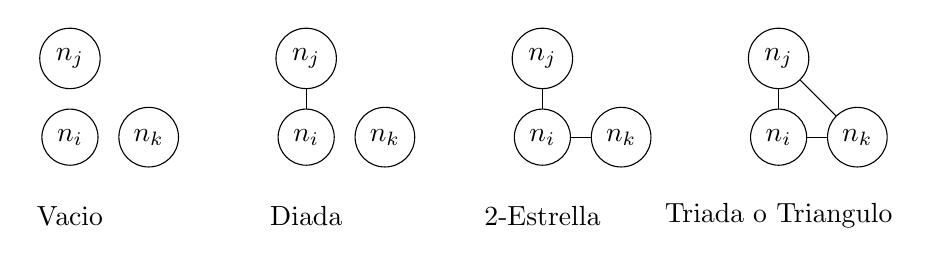
\begin{tikzpicture}[ scale=1]
\tikzset{vertex/.style = {shape=circle,draw,minimum size=2em}}
\tikzset{edge/.style = {->,> = latex}}


% vertices


\node[vertex] (g) at (0,6) {$n_j$};
\node[vertex] (h) at (0,5) {$n_i$};
\node[vertex] (i) at (1,5) {$n_k$};

\node[vertex] (j) at (3,6) {$n_j$};
\node[vertex] (k) at (3,5) {$n_i$};
\node[vertex] (l) at (4,5) {$n_k$};

\path[] (j) edge (k);

\node[vertex] (m) at (6,6) {$n_j$};
\node[vertex] (n) at (6,5) {$n_i$};
\node[vertex] (o) at (7,5) {$n_k$};

\path[] (n) edge (m);
\path[] (n) edge (o);


\node[vertex] (m1) at (9,6) {$n_j$};
\node[vertex] (n1) at (9,5) {$n_i$};
\node[vertex] (o1) at (10,5) {$n_k$};

\path[] (n1) edge (m1);
\path[] (m1) edge (o1);
\path[] (o1) edge (n1);


\node (w) at (0,4) {Vacio};
\node (x) at (3,4) {Diada};
\node (x) at (6,4) {2-Estrella};
\node (x) at (9,4) {Triada o Triangulo};

%\draw (4,4) node[cross=8pt,Grafo] {};

%\draw (0.2,8)--(3.8,8);



\end{tikzpicture}

\end{figure}
\end{minipage}

\begin{minipage}{.2\linewidth}
\begin{figure}[H]\centering

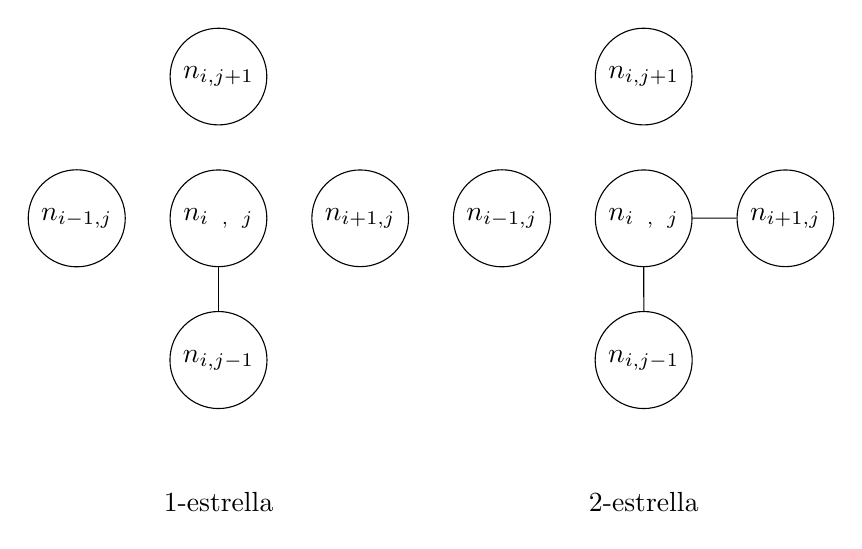
\begin{tikzpicture}[ scale=1.2]
\tikzset{vertex/.style = {shape=circle,draw,minimum size=1.5em}}
\tikzset{edge/.style = {->,> = latex}}
\tikzstyle{every node}=[font=\tiny]
\tikzstyle{every node}=[font=\fontsize{10}{10}\selectfont]

% vertices


\node[vertex] (g) at (0,3.5) {$n_{i,j-1}$};
\node[vertex] (h) at (0,5) {$n_{i\enskip, \enskip j}$};
\node[vertex] (i) at (1.5,5) {$n_{i+1,j}$};
\node[vertex] (j) at (-1.5,5) {$n_{i-1,j}$};
\node[vertex] (k) at (0,6.5) {$n_{i,j+1}$};

\path[] (g) edge (h);

\node[vertex] (g1) at (4.5,3.5) {$n_{i,j-1}$};
\node[vertex] (h1) at (4.5,5) {$n_{i\enskip, \enskip j}$};
\node[vertex] (i1) at (6,5) {$n_{i+1,j}$};
\node[vertex] (j1) at (3,5) {$n_{i-1,j}$};
\node[vertex] (k1) at (4.5,6.5) {$n_{i,j+1}$};

\path[] (g1) edge (h1);
\path[] (h1) edge (i1);


\node (w) at (0,2) {1-estrella};
\node (x) at (4.5,2) {2-estrella};

%\draw (4,4) node[cross=8pt,Grafo] {};

%\draw (0.2,8)--(3.8,8);

\end{tikzpicture}
\end{figure}
\end{minipage}

\begin{minipage}{.2\linewidth}
\begin{figure}[H]\centering

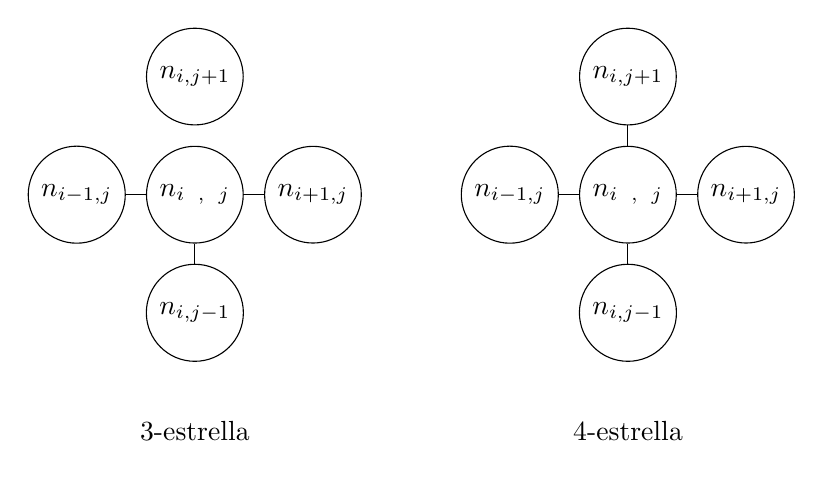
\begin{tikzpicture}[ scale=1]
\tikzset{vertex/.style = {shape=circle,draw,minimum size=1.5em}}
\tikzset{edge/.style = {->,> = latex}}
\tikzstyle{every node}=[font=\tiny]
\tikzstyle{every node}=[font=\fontsize{10}{10}\selectfont]

% vertices


\node[vertex] (g) at (1,3.5) {$n_{i,j-1}$};
\node[vertex] (h) at (1,5) {$n_{i\enskip, \enskip j}$};
\node[vertex] (i) at (2.5,5) {$n_{i+1,j}$};
\node[vertex] (j) at (-.5,5) {$n_{i-1,j}$};
\node[vertex] (k) at (1,6.5) {$n_{i,j+1}$};

\path[] (g) edge (h);
\path[] (j) edge (h);
\path[] (i) edge (h);

\node[vertex] (g1) at (6.5,3.5) {$n_{i,j-1}$};
\node[vertex] (h1) at (6.5,5) {$n_{i\enskip, \enskip j}$};
\node[vertex] (i1) at (8,5) {$n_{i+1,j}$};
\node[vertex] (j1) at (5,5) {$n_{i-1,j}$};
\node[vertex] (k1) at (6.5,6.5) {$n_{i,j+1}$};

\path[] (g1) edge (h1);
\path[] (j1) edge (h1);
\path[] (i1) edge (h1);
\path[] (k1) edge (h1);

\node (w) at (1,2) {3-estrella};
\node (x) at (6.5,2) {4-estrella};

%\draw (4,4) node[cross=8pt,Grafo] {};

%\draw (0.2,8)--(3.8,8);

\end{tikzpicture}
\end{figure}
\end{minipage}

\begin{minipage}{.2\linewidth}
\begin{figure}[H]\centering

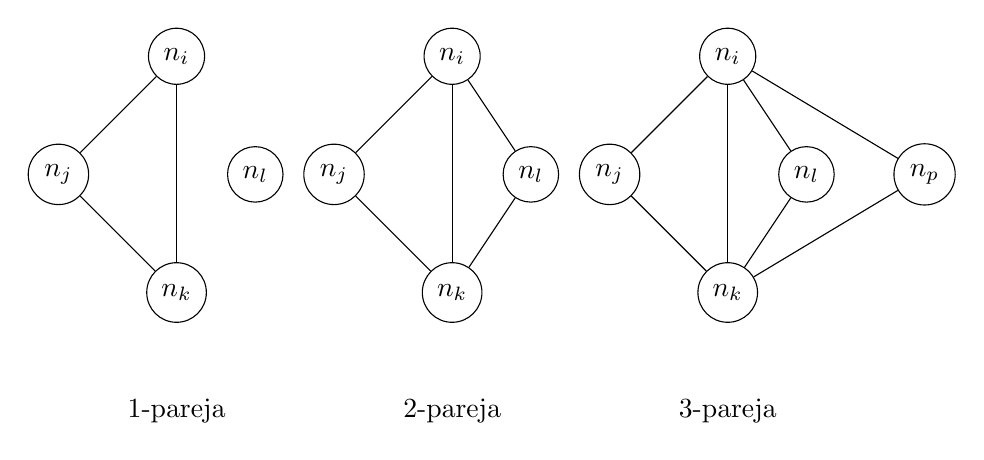
\begin{tikzpicture}[ scale=1]
\tikzset{vertex/.style = {shape=circle,draw,minimum size=1.5em}}
\tikzset{edge/.style = {->,> = latex}}
\tikzstyle{every node}=[font=\tiny]
\tikzstyle{every node}=[font=\fontsize{10}{10}\selectfont]

% vertices


\node[vertex] (g) at (1,3.5) {$n_{k}$};
\node[vertex] (j) at (-.5,5) {$n_{j}$};
\node[vertex] (k) at (1,6.5) {$n_{i}$};

\node[vertex] (i) at (2,5) {$n_{l}$};


\path[] (g) edge (j);
\path[] (j) edge (k);
\path[] (k) edge (g);


\node[vertex] (g) at (4.5,3.5) {$n_{k}$};
\node[vertex] (j) at (3,5) {$n_{j}$};
\node[vertex] (k) at (4.5,6.5) {$n_{i}$};

\node[vertex] (i) at (5.5,5) {$n_{l}$};


\path[] (g) edge (j);
\path[] (j) edge (k);
\path[] (k) edge (g);
\path[] (g) edge (i);
\path[] (k) edge (i);

\node[vertex] (g) at (8,3.5) {$n_{k}$};
\node[vertex] (j) at (6.5,5) {$n_{j}$};
\node[vertex] (k) at (8,6.5) {$n_{i}$};

\node[vertex] (i) at (9,5) {$n_{l}$};
\node[vertex] (i2) at (10.5,5) {$n_{p}$};


\path[] (g) edge (j);
\path[] (j) edge (k);
\path[] (k) edge (g);
\path[] (g) edge (i);
\path[] (k) edge (i);
\path[] (g) edge (i2);
\path[] (k) edge (i2);

\node (w) at (1,2) {1-pareja};
\node (x) at (4.5,2) {2-pareja};
\node (x1) at (8,2) {3-pareja};

%\draw (4,4) node[cross=8pt,Grafo] {};

%\draw (0.2,8)--(3.8,8);

\end{tikzpicture}
\end{figure}
\end{minipage}